\section{Introduction}
End-to-end automatic speech recognition (ASR) systems based on neural networks have seen large improvements in recent years.
Recurrent neural networks (RNNs) have been the de-facto choice for ASR~\cite{chiu2018state, rao2017exploring, Ryan19, tara2020} as they can model the temporal dependencies in the audio sequences effectively \cite{graves2012sequence}. Recently, the Transformer architecture based on self-attention~\cite{vaswani2017attention, zhang2020transformer} has enjoyed widespread adoption for modeling sequences due to its ability to capture long distance interactions and the high training efficiency. Alternatively, convolutions have also been successful for ASR~\cite{li2019jasper, kriman2019quartznet, han2020contextnet, sainath2013deep, abdel2014convolutional}, which capture local context progressively via a local receptive field layer by layer. 


However, models with self-attention or convolutions each has its limitations. While Transformers are good at modeling long-range global context, they are less capable to extract fine-grained local feature patterns. Convolution neural networks (CNNs), on the other hand, exploit local information and are used as the de-facto computational block in vision. They learn shared position-based kernels over a local window which maintain translation equivariance and are able to capture features like edges and shapes. One limitation of using local connectivity is that you need many more layers or parameters to capture global information. To combat this issue, contemporary work ContextNet~\cite{han2020contextnet} adopts the squeeze-and-excitation module~\cite{hu2018squeeze} in each residual block to capture longer context. However, it is still limited in capturing dynamic global context as it only applies a global averaging over the entire sequence.

Recent works have shown that combining convolution and self-attention improves over using them individually~\cite{bello2019attention}. Together, they are able to learn both position-wise local features, and use content-based global interactions. Concurrently, papers like \cite{yang2019convolutional, yu2018qanet} have augmented self-attention with relative position based information that maintains equivariance. Wu et al. \cite{wu2020lite} proposed a multi-branch architecture with splitting the input into two branches: self-attention and convolution; and concatenating their outputs. Their work targeted mobile applications and showed improvements in machine translation tasks.

\begin{figure}[t]
    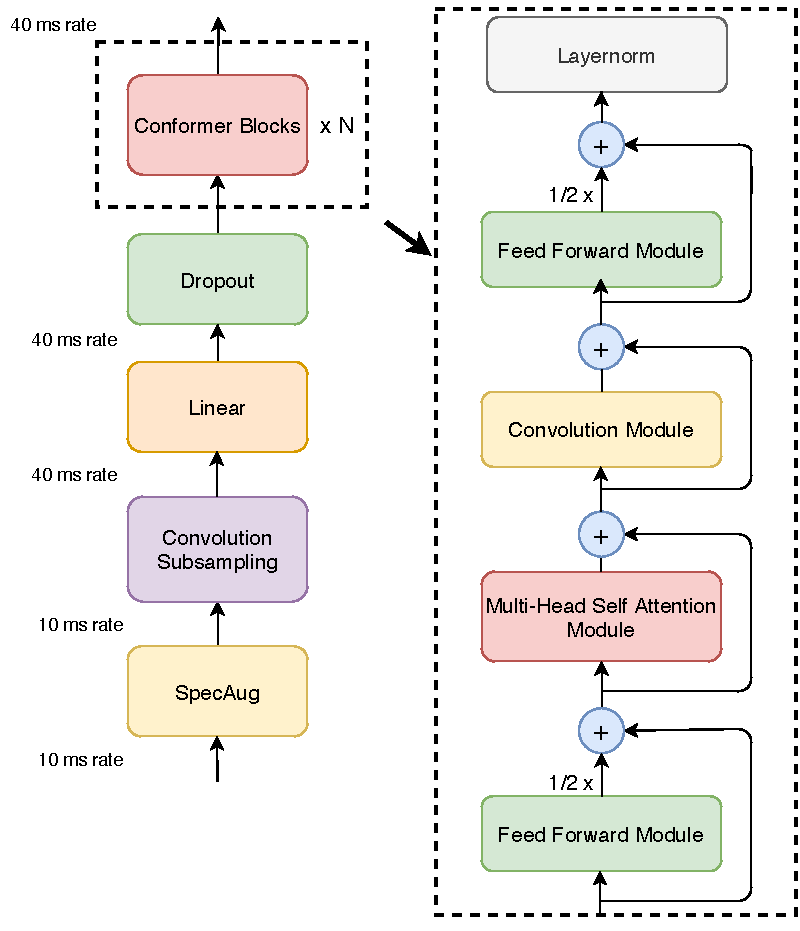
\includegraphics[width=0.8\columnwidth]{figure/conformer_new.pdf}
    \caption{\textbf{Conformer encoder model architecture.} Conformer comprises of two macaron-like feed-forward layers with half-step residual connections sandwiching the multi-headed self-attention and convolution modules. This is followed by a post layernorm.}
    \label{fig:conformer}
\end{figure}


\label{sec:model:convolution}
\begin{figure*}
    \centering
    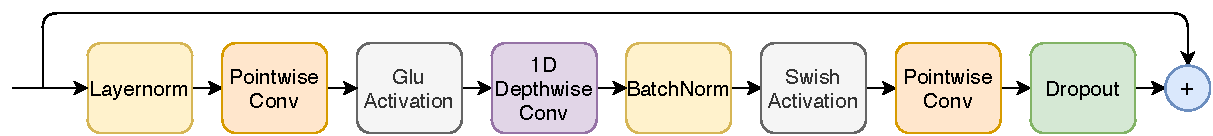
\includegraphics[width=0.7\textwidth]{figure/conv_block.pdf}
    \caption{\textbf{Convolution module.} The convolution module contains a pointwise convolution with an expansion factor of 2 projecting the number of channels with a GLU activation layer, followed by a 1-D Depthwise convolution. The 1-D depthwise conv is followed by a Batchnorm and then a swish activation layer.  }
    \label{fig:conv}
\end{figure*}


In this work, we study how to organically combine convolutions with self-attention in ASR models. We hypothesize that both global and local interactions are important for being parameter efficient. To achieve this, we propose a novel combination of self-attention and convolution will achieve the best of both worlds -- self-attention learns the global interaction whilst the convolutions efficiently capture the relative-offset-based local correlations.
%
Inspired by Wu et al. \cite{wu2020lite, lu2019understanding}, we introduce a novel combination of self-attention and convolution, sandwiched between a pair feed forward modules,  as illustrated in Fig~\ref{fig:conformer}.  

Our proposed model, named Conformer, achieves state-of-the-art results on LibriSpeech, outperforming the previous best published Transformer Transducer \cite{zhang2020transformer} by 15\% relative improvement on the testother dataset with an external language model. We present three models based on model parameter limit constraints of 10M , 30M and 118M.
Our 10M model shows an improvement when compared to similar sized contemporary work \cite{han2020contextnet} with 2.7\%/6.3\% on test/testother datasets. 
Our medium 30M parameters-sized model already outperforms  transformer transducer published in  \cite{zhang2020transformer} which uses 139M model parameters.
With the big 118M parameter model, we are able to achieve 2.1\%/4.3\% without using language models and 1.9\%/3.9\% with an external language model.

We further carefully study the effects of the number of attention heads, convolution kernel sizes, activation functions, placement of feed-forward layers, and different strategies of adding convolution modules to a Transformer-based network, and shed light on how each contributes to the accuracy improvements.